\documentclass[]{book}
\usepackage{lmodern}
\usepackage{amssymb,amsmath}
\usepackage{ifxetex,ifluatex}
\usepackage{fixltx2e} % provides \textsubscript
\ifnum 0\ifxetex 1\fi\ifluatex 1\fi=0 % if pdftex
  \usepackage[T1]{fontenc}
  \usepackage[utf8]{inputenc}
\else % if luatex or xelatex
  \ifxetex
    \usepackage{mathspec}
  \else
    \usepackage{fontspec}
  \fi
  \defaultfontfeatures{Ligatures=TeX,Scale=MatchLowercase}
\fi
% use upquote if available, for straight quotes in verbatim environments
\IfFileExists{upquote.sty}{\usepackage{upquote}}{}
% use microtype if available
\IfFileExists{microtype.sty}{%
\usepackage{microtype}
\UseMicrotypeSet[protrusion]{basicmath} % disable protrusion for tt fonts
}{}
\usepackage[margin=1in]{geometry}
\usepackage{hyperref}
\hypersetup{unicode=true,
            pdftitle={Case Studies in Reproducible Research: a spring seminar at UCSC},
            pdfauthor={Eric C. Anderson, Kristen C. Ruegg, Tina Cheng, and the students of EEB 295},
            pdfborder={0 0 0},
            breaklinks=true}
\urlstyle{same}  % don't use monospace font for urls
\usepackage{natbib}
\bibliographystyle{apalike}
\usepackage{color}
\usepackage{fancyvrb}
\newcommand{\VerbBar}{|}
\newcommand{\VERB}{\Verb[commandchars=\\\{\}]}
\DefineVerbatimEnvironment{Highlighting}{Verbatim}{commandchars=\\\{\}}
% Add ',fontsize=\small' for more characters per line
\usepackage{framed}
\definecolor{shadecolor}{RGB}{248,248,248}
\newenvironment{Shaded}{\begin{snugshade}}{\end{snugshade}}
\newcommand{\KeywordTok}[1]{\textcolor[rgb]{0.13,0.29,0.53}{\textbf{{#1}}}}
\newcommand{\DataTypeTok}[1]{\textcolor[rgb]{0.13,0.29,0.53}{{#1}}}
\newcommand{\DecValTok}[1]{\textcolor[rgb]{0.00,0.00,0.81}{{#1}}}
\newcommand{\BaseNTok}[1]{\textcolor[rgb]{0.00,0.00,0.81}{{#1}}}
\newcommand{\FloatTok}[1]{\textcolor[rgb]{0.00,0.00,0.81}{{#1}}}
\newcommand{\ConstantTok}[1]{\textcolor[rgb]{0.00,0.00,0.00}{{#1}}}
\newcommand{\CharTok}[1]{\textcolor[rgb]{0.31,0.60,0.02}{{#1}}}
\newcommand{\SpecialCharTok}[1]{\textcolor[rgb]{0.00,0.00,0.00}{{#1}}}
\newcommand{\StringTok}[1]{\textcolor[rgb]{0.31,0.60,0.02}{{#1}}}
\newcommand{\VerbatimStringTok}[1]{\textcolor[rgb]{0.31,0.60,0.02}{{#1}}}
\newcommand{\SpecialStringTok}[1]{\textcolor[rgb]{0.31,0.60,0.02}{{#1}}}
\newcommand{\ImportTok}[1]{{#1}}
\newcommand{\CommentTok}[1]{\textcolor[rgb]{0.56,0.35,0.01}{\textit{{#1}}}}
\newcommand{\DocumentationTok}[1]{\textcolor[rgb]{0.56,0.35,0.01}{\textbf{\textit{{#1}}}}}
\newcommand{\AnnotationTok}[1]{\textcolor[rgb]{0.56,0.35,0.01}{\textbf{\textit{{#1}}}}}
\newcommand{\CommentVarTok}[1]{\textcolor[rgb]{0.56,0.35,0.01}{\textbf{\textit{{#1}}}}}
\newcommand{\OtherTok}[1]{\textcolor[rgb]{0.56,0.35,0.01}{{#1}}}
\newcommand{\FunctionTok}[1]{\textcolor[rgb]{0.00,0.00,0.00}{{#1}}}
\newcommand{\VariableTok}[1]{\textcolor[rgb]{0.00,0.00,0.00}{{#1}}}
\newcommand{\ControlFlowTok}[1]{\textcolor[rgb]{0.13,0.29,0.53}{\textbf{{#1}}}}
\newcommand{\OperatorTok}[1]{\textcolor[rgb]{0.81,0.36,0.00}{\textbf{{#1}}}}
\newcommand{\BuiltInTok}[1]{{#1}}
\newcommand{\ExtensionTok}[1]{{#1}}
\newcommand{\PreprocessorTok}[1]{\textcolor[rgb]{0.56,0.35,0.01}{\textit{{#1}}}}
\newcommand{\AttributeTok}[1]{\textcolor[rgb]{0.77,0.63,0.00}{{#1}}}
\newcommand{\RegionMarkerTok}[1]{{#1}}
\newcommand{\InformationTok}[1]{\textcolor[rgb]{0.56,0.35,0.01}{\textbf{\textit{{#1}}}}}
\newcommand{\WarningTok}[1]{\textcolor[rgb]{0.56,0.35,0.01}{\textbf{\textit{{#1}}}}}
\newcommand{\AlertTok}[1]{\textcolor[rgb]{0.94,0.16,0.16}{{#1}}}
\newcommand{\ErrorTok}[1]{\textcolor[rgb]{0.64,0.00,0.00}{\textbf{{#1}}}}
\newcommand{\NormalTok}[1]{{#1}}
\usepackage{longtable,booktabs}
\usepackage{graphicx,grffile}
\makeatletter
\def\maxwidth{\ifdim\Gin@nat@width>\linewidth\linewidth\else\Gin@nat@width\fi}
\def\maxheight{\ifdim\Gin@nat@height>\textheight\textheight\else\Gin@nat@height\fi}
\makeatother
% Scale images if necessary, so that they will not overflow the page
% margins by default, and it is still possible to overwrite the defaults
% using explicit options in \includegraphics[width, height, ...]{}
\setkeys{Gin}{width=\maxwidth,height=\maxheight,keepaspectratio}
\IfFileExists{parskip.sty}{%
\usepackage{parskip}
}{% else
\setlength{\parindent}{0pt}
\setlength{\parskip}{6pt plus 2pt minus 1pt}
}
\setlength{\emergencystretch}{3em}  % prevent overfull lines
\providecommand{\tightlist}{%
  \setlength{\itemsep}{0pt}\setlength{\parskip}{0pt}}
\setcounter{secnumdepth}{5}
% Redefines (sub)paragraphs to behave more like sections
\ifx\paragraph\undefined\else
\let\oldparagraph\paragraph
\renewcommand{\paragraph}[1]{\oldparagraph{#1}\mbox{}}
\fi
\ifx\subparagraph\undefined\else
\let\oldsubparagraph\subparagraph
\renewcommand{\subparagraph}[1]{\oldsubparagraph{#1}\mbox{}}
\fi

%%% Use protect on footnotes to avoid problems with footnotes in titles
\let\rmarkdownfootnote\footnote%
\def\footnote{\protect\rmarkdownfootnote}

%%% Change title format to be more compact
\usepackage{titling}

% Create subtitle command for use in maketitle
\newcommand{\subtitle}[1]{
  \posttitle{
    \begin{center}\large#1\end{center}
    }
}

\setlength{\droptitle}{-2em}
  \title{Case Studies in Reproducible Research: a spring seminar at UCSC}
  \pretitle{\vspace{\droptitle}\centering\huge}
  \posttitle{\par}
  \author{Eric C. Anderson, Kristen C. Ruegg, Tina Cheng, and the students of EEB
295}
  \preauthor{\centering\large\emph}
  \postauthor{\par}
  \predate{\centering\large\emph}
  \postdate{\par}
  \date{2017-04-21}

\usepackage{booktabs}
\usepackage{amsthm}
\makeatletter
\def\thm@space@setup{%
  \thm@preskip=8pt plus 2pt minus 4pt
  \thm@postskip=\thm@preskip
}
\makeatother

\usepackage{amsthm}
\newtheorem{theorem}{Theorem}[chapter]
\newtheorem{lemma}{Lemma}[chapter]
\theoremstyle{definition}
\newtheorem{definition}{Definition}[chapter]
\newtheorem{corollary}{Corollary}[chapter]
\newtheorem{proposition}{Proposition}[chapter]
\theoremstyle{definition}
\newtheorem{example}{Example}[chapter]
\theoremstyle{remark}
\newtheorem*{remark}{Remark}
\begin{document}
\maketitle

{
\setcounter{tocdepth}{1}
\tableofcontents
}
\chapter{Course Overview}\label{course-overview}

This is the home of the notes for a proposed course in data analysis and
reproducible research using R, Rstudio, and GitHub.

The seminar is called, ``Case Studies in Reproducible Research,'' but we
utter that title with the caveat that, although the organizers have
quite a few case studies they could spin up for this course, the case
studies we will be studying in this course are going to be actual
research projects that \emph{you}---the participants---are working on.
You're gonna bring 'em, and we are going to collectively help you
wrassle them into a reasonable and reproducible data analysis. In the
process we will touch on a number of elements of data analysis with R.

We will be working through a healthy chunk of the material in Garrett
Grolemund and Hadley Wickham's book, \href{http://r4ds.had.co.nz/}{R for
Data Science}, which is readable for free at the link above. We intend
to use a handful of our own data sets each week to illustrate points
from the book and show the material in action on real data sets.

This is not intended as a ``first course in R''. Students coming to the
course should have at least a modicum of familiarity with using R, and
we will launch more directly into using the tools of the
\href{http://tidyverse.org/}{tidyverse}. EEB students with little or no
experience in R might be interested in sitting in with Giacomo
Bernardi's lab group on Mondays at 3PM in the COH library. They are
conducting a Bio 295 seminar, working through ``a super basic book that
takes the very first steps into R.''

For the interested, these materials were all prepared using RStudio's
\href{https://bookdown.org/}{bookdown} package. The RStudio project in
which it lives is hosted on eriq's GitHub page
\href{https://github.com/eriqande/rep-res-eeb-2017}{here}

\section{Meeting Times, Location,
Requirements}\label{meeting-times-location-requirements}

Intended to be Friday afternoons, 1:45--3:15 PM in the
library/conference room at Long Marine Lab.

Students must bring a laptop to do examples during the seminar, and all
students are expected to have a data set that they are in the midst of
analyzing (or upon which they hope to commence analysis soon!) for a
research project. We will

\section{The origin of this seminar}\label{the-origin-of-this-seminar}

The idea for this course was floated by Tina Cheng who was planning to
lead a seminar in spring 2017 based in part on Eric C. Anderson's
\href{http://eriqande.github.io/rep-res-web/}{``Reproducible Research
Course''}, taught at the Southwest Fisheries Science Center in the fall
of 2014. Although going over those notes might have been a reasonable
exercise, it turns out that a lot has changed in the world of data
analysis since fall 2014, and the notes from that course are, today, a
little bit dated.

We have been particularly excited by the ascendancy of Hadley Wickham's
\href{http://tidyverse.org/}{tidyverse} approach to data analysis, and
the tremendous development of a variety of tools developed by
\href{https://www.rstudio.com/}{RStudio} for integrating report
generation and data analysis into reproducible workflows. In fact, Eric
has been saying for the last year that if he were to teach another
course on data analysis it would be structured completely differently
than his \href{http://eriqande.github.io/rep-res-web/}{``Reproducible
Research Course''}. So, it was clearly time for him to stop talking and
help put together an updated and different course.

At the same time, in working on our own projects and in helping others,
we have consistently found that the most effective way for anyone to
learn data analysis is to ensure that it is immediately relevant to
whatever ongoing research project is currently consuming them.
Therefore, in the current seminar, we are hoping to spend at least half
of our time ``workshopping'' the data sets that seminar participants are
actually involved in analyzing. Together we will help students wrestle
their data, analyses, and ideas into a single, well-organized RStudio
project under version control with git. Therefore, every student should
come to this course with a data set and an associated analysis project.

\section{Course Organizers}\label{course-organizers}

\begin{description}
\item[Kristen C. Ruegg]
Kristen is a conservation geneticist who specializes in the application
of genome-wide data to understand population level processes and inform
management, with a particular focus on migratory birds. She has has been
enlightened to the powers of the ``tidyverse'' over the last couple of
years (mostly through the constant insistence of her enthusiastic
husband Eric Anderson) and is looking forward to becoming more fluid in
its application over the course of the quarter. Her main role in this
course will be to help with the course design and logistics and help
reign Eric in when he has started to orbit into some obscure realm of
statistical nuance.
\item[Eric C. Anderson]
Eric trained as a statistician who specializes in genetic data. Since
2003 he has worked at the NMFS Southwest Fisheries Science Center in
Santa Cruz. Although much of his statistical research involves the
development of computationally intensive methods for specialized
analyses of genetic data, he has been involved in a variety of data
analysis projects at NMFS and with collaborators worldwide. Eric was an
early adherent to reproducible research principles and continues, as
such, performing most of his research and data analysis in the open and
publicly available on GitHub (find his GitHub page
\href{https://github.com/eriqande}{here}). In 2014, he taught the
\href{http://eriqande.github.io/rep-res-web/}{``Reproducible Research
Course''} at NMFS, and is excited to provide an updated version,
focusing more, this time, on the recently developed ``tidyverse''.
\item[Tina Cheng]
Tina is a graduate student in EEB. She is going to be leading the
session during the first week of the course when Kristen and Eric are
still on spring break, and then she is going to be joining in on the fun
with us for the remainder of the quarter until she has to travel off to
Baja, TA-ing the ``supercourse'' during the last four weeks of the
quarter.
\end{description}

\section{Course Goals}\label{course-goals}

The goal of this course is for scientists, researchers, and students to
learn to:

\begin{itemize}
\tightlist
\item
  properly store, manage, and distribute their data in a \emph{tidy}
  format
\item
  consolidate their digital research materials and analyses into
  well-organized RStudio projects.
\item
  use the tools of the tidyverse to manipulate and analyze those data
  sets
\item
  integrate data analysis with report generation and article preparation
  using the Rmarkdown format and using
  \href{http://rmarkdown.rstudio.com/r_notebooks.html}{R Notebooks}
\item
  use git version control software and GitHub to effectively manage data
  and source code, collaborate efficiently with other researchers, and
  neatly package their research.
\end{itemize}

By the end of the course, the hope is that we will all have mastered
strategies allowing us to use the above-listed, freely-available and
open-source tools for conducting research in a reproducible fashion. The
ideal we will be striving for is to be able to start from a raw data set
and then write a computer program that conducts all the cleaning,
manipulation, and analysis of the data, and presentation of the results,
in an automated fashion. Carrying out analysis and report-generation in
this way carries a number of advantages to the researcher:

\begin{enumerate}
\def\labelenumi{\arabic{enumi}.}
\tightlist
\item
  Newly-collected data can be integrated easily into your analysis.
\item
  If a mistake is found in one section of your analysis, it is not
  terribly onerous to correct it and then re-run all the downstream
  analyses.
\item
  Revising a manuscript to address referee comments can be done quickly.
\item
  Years after publication, the exact steps taken to analyze the data
  will still be available should anyone ask you how, exactly, you did an
  analysis!
\item
  If you have to conduct similar analyses and produce similar reports on
  a regular bias with new data each time, you might be able to do this
  readily by merely updating your data and then automatically producing
  the entire report.
\item
  If someone finds an error in your work, they can fix it and then
  easily show you exactly what they did to fix it.
\end{enumerate}

Additionally, packaging one's research in a reproducible fashion is
beneficial to the research community. Others that would like to confirm
your results can do so easily. If someone has concerns about exactly how
a particular analysis was carried out, they can find the precise details
in the code that you wrote to do it. Someone wanting to apply your
methods to their own data can easily do so, and, finally, if we are all
transparent and open about the methods that we use, then everyone can
learn more quickly from their colleagues.

In many fields today, publication of research requires the submission of
the original data to a publicly-available data repository. Currently,
several journals require that all analyses be packaged in a clear and
transparent fashion for easy reproduction of the results, and I predict
that trend will continue until most, if not all, journals will require
that data analyses be available in easily reproduced formats. This
course will help scientists prepare themselves for this eventuality. In
the process, you will probably find that conducting your research in a
reproducible fashion helps you work more efficiently (and perhaps even
more enjoyably!)

\section{Weekly Syllabus}\label{weekly-syllabus}

\subsection{Week 1 --- Introduction and Getting Your Workspace Set
Up}\label{week-1-introduction-and-getting-your-workspace-set-up}

\begin{itemize}
\tightlist
\item
  At the end of this session we want to make sure that everyone has R,
  RStudio, and Git installed on their systems, and that they are working
  as expected.
\item
  Additionally, everyoneshould have a free account on GitHub.
\item
  And finally we need everyone's email address.
\end{itemize}

Some things to do:

\begin{itemize}
\tightlist
\item
  Get Rstudio cheat Sheets!
\item
  Assemble data into a project
\item
  Get private GitHub repos
\end{itemize}

Eric! You need to make an example project repo.

\subsection{Week 2 --- RStudio project organization; using git and
GitHub; Quick
RMarkdown}\label{week-2-rstudio-project-organization-using-git-and-github-quick-rmarkdown}

After this, students are going to have to put their own data into their
own repositories and write a README.Rmd and make a README.md out of it.

\subsection{Week 3 --- Tibbles. Reading data in. Data
rectangling}\label{week-3-tibbles.-reading-data-in.-data-rectangling}

\begin{itemize}
\tightlist
\item
  Reading data into the data frames.
\item
  read.table and read.csv
\item
  tibbles
\item
  The readr package
\item
  Data types in the different columns and quick data sanity checks.
\item
  A few different gotcha's
\item
  Saving and reading data in R formats. \texttt{saveRDS} and
  \texttt{readRDS}.
\end{itemize}

\subsection{Week 4 ---}\label{week-4}

\chapter{Week One Meeting}\label{week1}

Tina is going to be helping everyone get their systems all set up. After
that we will have everyone clone an RStudio project from GitHub to see
how easy that is.

\section{Software Installation}\label{software-installation}

\begin{enumerate}
\def\labelenumi{\arabic{enumi}.}
\item
  \textbf{RStudio:} We want the latest ``development'' version of
  RStudio becuase it has features that we may want to use during this
  course. Get it from
  \url{https://www.rstudio.com/products/rstudio/download/preview/} and
  install the appropriate one for your OS.
\item
  \textbf{R:} Let's make sure that we are all using the latest version
  of R. On March 7, 2017, version 3.3.3 was released. Go to
  \url{https://cran.r-project.org/} and find the download link for your
  computer system. Download it and install it.
\item
  \textbf{bookdown:} This package is what I used to create these course
  notes. Getting it automatically installs a lot of other packages that
  are useful for authoring reproducible research. We want the latest
  development version, which can be obtained from GitHub by issuing the
  following commans at the R prompt (i.e.~in the console window of
  RStudio:)

\begin{Shaded}
\begin{Highlighting}[]
\KeywordTok{install.packages}\NormalTok{(}\StringTok{"devtools"}\NormalTok{)  }
\NormalTok{devtools::}\KeywordTok{install_github}\NormalTok{(}\StringTok{"rstudio/bookdown"}\NormalTok{)}
\end{Highlighting}
\end{Shaded}
\item
  Install \textbf{other packages} that we are going to be needing in the
  first few weeks. If you don't know how to install packages, ask Tina
  and she can show you. Install: \texttt{tidyverse}, and
  \texttt{stringr}.
\item
  Make sure that \textbf{git} is up and running on your system.

  \begin{itemize}
  \item
    If you are using a Mac with a reasonably new OS, you should be able
    to just open the Terminal application
    (\texttt{/Applications/Utilities/Terminal}) and type ``git'' at the
    command line. If you have \texttt{git} it will say something that
    starts like:

\begin{Shaded}
\begin{Highlighting}[]
    \KeywordTok{usage}\NormalTok{: git [--version] [--help] [-C }\KeywordTok{<}\NormalTok{path}\KeywordTok{>}\NormalTok{] [-c name=value]}
   \NormalTok{[}\KeywordTok{--exec-path}\NormalTok{[=}\KeywordTok{<}\NormalTok{path}\KeywordTok{>}\NormalTok{]] [--html-path] [--man-path] [--info-path]}
   \NormalTok{[}\KeywordTok{-p} \KeywordTok{|} \KeywordTok{--paginate} \KeywordTok{|} \KeywordTok{--no-pager}\NormalTok{] [--no-replace-objects] [--bare]}
   \NormalTok{[}\KeywordTok{--git-dir}\NormalTok{=}\KeywordTok{<}\NormalTok{path}\KeywordTok{>}\NormalTok{] [--work-tree=}\KeywordTok{<}\NormalTok{path}\KeywordTok{>}\NormalTok{] [--namespace=}\KeywordTok{<}\NormalTok{name}\KeywordTok{>}\NormalTok{]}
   \KeywordTok{<command>} \NormalTok{[}\KeywordTok{<}\NormalTok{args}\KeywordTok{>}\NormalTok{]}

\KeywordTok{These} \NormalTok{are common Git commands used in various situations:}

\KeywordTok{start} \NormalTok{a working area (see also: git help tutorial)}
   \KeywordTok{clone}      \NormalTok{Clone a repository into a new directory}
   \KeywordTok{etc.} \NormalTok{etc. etc.}
\end{Highlighting}
\end{Shaded}

    If you do not have \texttt{git} then it should pop up a little thing
    asking if you would like to install a reduced set of developer
    tools. You do. Click OK. \textbf{NOTE} Instead of a pop up it might
    say something like, ``xcrun Error: invalid active developer path.
    etc. etc\ldots{}''. In that case, you can install a fresh set of
    command line tools by typing this at the command line:

\begin{verbatim}
xcode-select --install
\end{verbatim}
  \item
    If you are using a PC, I can't be as much help, but you can find
    links with instructions on how to download \texttt{git} for a PC
    \href{https://support.rstudio.com/hc/en-us/articles/200532077-Version-Control-with-Git-and-SVN}{here}.
  \item
    If you are using Linux then we will assume you know how to get
    \texttt{git} or that you already have it.
  \end{itemize}
\end{enumerate}

\section{Get an account on GitHub}\label{get-an-account-on-github}

If you don't already have an account on GitHub, go to \url{github.com}
and click the ``sign up'' link near upper right of the page. It is
pretty self-explanatory. Go ahead and get a \textbf{free} account. There
is nothing to pay for here!

\subsection{Private repositories}\label{private-repositories}

\emph{If you are a graduate student} and you do not feel comfortable
posting your data on a public site like GitHub, then you should request
some private repositories from GitHub. GitHub has a great deal for
academic users like students: free private repositories. Please go to
\url{https://education.github.com/pack} to sign up for your free student
pack.

\section{Open an RStudio Project from
GitHub}\label{open-an-rstudio-project-from-github}

I am going to have everyone use RStudio and GitHub to clone and open an
RStudio project that I prepared as a template so that people can see how
I would like them to start putting together their own projects.

To open this project, from RStudio, go to the menu option
``File-\textgreater{}New Project\ldots{}''. Then from the resulting
dialog, choose ``Version Control''. Then choose ``Git''. Then it asks
for a ``repository URL''. Supply this:
\texttt{https://github.com/eriqande/rep-res-coho-example} and leave the
``Project Directory Name'' empty. And then choose a directory in which
to put it and click OK.

Bam! That will pull the RStudio project off of GitHub, make a local
clone of it on your hard drive and open.

Once you have done that. Open \texttt{README.Rmd} within the project,
and click the ``knit'' button which should be present near the top left
of the editor window.

That is how you convert an R Markdown README to README.md which is easy
to read and see on GitHub.

If you want to see what the project repository looks like on GitHub,
have a look at \url{https://github.com/eriqande/rep-res-coho-example}.

\section{Assignment for next week: Create an RStudio Project with Your
Own
Data}\label{assignment-for-next-week-create-an-rstudio-project-with-your-own-data}

Your mission for the following week---i.e., please have this done (or as
done as you can get it) by Friday, April 14, 2017---is to prepare an
RStudio project with your own data set, and provide some background
about the data and the ways that you would like to analyze it. The
``rep-res-coho-example'' is an example of what I have in mind for this.
You should use the README.Rmd from that project as a template for your
own README.Rmd. (To do this you can just copy the README.Rmd file into
the top level of your project directory and then edit it to reflect your
own data and project.)

To do all this you are going to want to make your own project. Do that
like this:

\begin{enumerate}
\def\labelenumi{\arabic{enumi}.}
\tightlist
\item
  In RStudio, choose ``File-\textgreater{}New Project\ldots{}''
\item
  Then choose ``New Directory'' and then choose ``Empty Project''
\item
  In the next dialog, choose a name (\emph{it is best to use only
  letters, numbers, dashes, and underscores, and include no spaces in
  the name}) for it \textbf{and be sure to click the ``Create a git
  repository'' button}.\\
\item
  Then click ``Create Project''.
\end{enumerate}

That should give you a new project. Here are some guidelines for putting
your own data in there

\begin{itemize}
\tightlist
\item
  Put all of your data in a directory named \texttt{data} in your
  project.
\item
  CSV (comma separated values) is probably the best format to use. It is
  text-readable without proprietary software (unlike an Excel file);
  however if you need to look at it in a tabular way with Excel, (gasp),
  you can do that easily. Tab-delimited text works if you have that, but
  CSV is preferred.
\item
  Use only letters, numbers, dashes, and underscores for the file names,
  (and periods for their extensions, i.e., \texttt{.csv})
\item
  Give a brief description of your data in the README.Rmd.
\end{itemize}

\section{Reading for next week}\label{week2reading}

This week (before Friday, April 14, 2017), please read the following
sections of the R for Data Science book

\begin{itemize}
\tightlist
\item
  \href{http://r4ds.had.co.nz/workflow-basics.html}{Workflow basics}:
  super basic review on how R works.
\item
  \href{http://r4ds.had.co.nz/workflow-projects.html}{Workflow:
  projects}: info about organizing RStudio projects.
\item
  \href{http://r4ds.had.co.nz/workflow-scripts.html}{Workflow: scripts}:
  how to evaluate code in scripts.
\item
  \href{http://r4ds.had.co.nz/tibbles.html}{tibbles}: a streamlined data
  frame format.
\item
  \href{http://r4ds.had.co.nz/data-import.html}{data import} This is our
  key reading for the week.
\end{itemize}

When you are done with the \emph{Data Import} reading, take a whack at
writing some code to read the data files in your project into a variable
(or several variables).

\chapter{Week Two Meeting}\label{week2}

For this week, everyone should have completed the reading listed in
Section \ref{week2reading}. And everyone should have at least been
trying to set up an RStudio Project with their own data in it, and given
a whack at reading their data into a variable.

\section{Workflow and Project Recap}\label{workflow-and-project-recap}

\subsection{Workflow: basics}\label{workflow-basics}

\subsubsection{Style}\label{style}

I just want to reiterate a few things that might seem minor, but are
stylistically important in the long run.

\begin{enumerate}
\def\labelenumi{\arabic{enumi}.}
\tightlist
\item
  Don't use \texttt{=} for assignment. Use \texttt{\textless{}-}. On a
  Mac use Option-``-'' to get that more quickly.

  \begin{itemize}
  \item
    Hey! Note that you \emph{do} use \texttt{=} (and \textbf{only}
    \texttt{=}) for \emph{passing values to function arguments}.

\begin{Shaded}
\begin{Highlighting}[]
\CommentTok{# do this:}
\NormalTok{my_variable <-}\StringTok{ }\DecValTok{10}

\CommentTok{# don't do this (it works but is not good style)}
\NormalTok{my_variable =}\StringTok{ }\DecValTok{10}


\CommentTok{# do this}
\NormalTok{result <-}\StringTok{ }\KeywordTok{my_function}\NormalTok{(}\DataTypeTok{arg1 =} \DecValTok{10}\NormalTok{, }\DataTypeTok{arg2 =} \StringTok{"foo"}\NormalTok{)}

\CommentTok{# don't do this (it might return a results, but will likely be incorrect)}
\NormalTok{result <-}\StringTok{ }\KeywordTok{my_function}\NormalTok{(arg1 <-}\StringTok{ }\DecValTok{10}\NormalTok{, arg2 <-}\StringTok{ "foo"}\NormalTok{)}

\CommentTok{# for example, figure out how this fails:}
\KeywordTok{matrix}\NormalTok{(data <-}\StringTok{ }\DecValTok{1}\NormalTok{:}\DecValTok{10}\NormalTok{, nrow <-}\StringTok{ }\DecValTok{5}\NormalTok{, byrow <-}\StringTok{ }\OtherTok{TRUE}\NormalTok{)}
\end{Highlighting}
\end{Shaded}
  \end{itemize}
\item
  Put spaces around both sides of \texttt{=}, and \texttt{\textless{}-},
  and other mathematical operators like \texttt{+}, \texttt{-},
  \texttt{*}, etc.
\item
  Put spaces after commas.
\item
  Use R-Studio's magical \texttt{Cmd-i} keyboard shortcut to
  automatically indent highlighted code.
\item
  If you want to really geek out, Hadley shares his style tips more
  completely in his \href{http://adv-r.had.co.nz/Style.html}{Advanced R
  Programming} book.
\end{enumerate}

This might seem pedantic, but adhering to these conventions makes it
much easier for people to read your code.

\subsubsection{TAB-completion}\label{tab-completion}

This is HUGE!! Start developing a twitchy left pinky now!

TAB early; TAB often!

Note that that completions of R code in the console or in the source
window are context dependent:

\begin{itemize}
\tightlist
\item
  variables in global environment
\item
  Functions
\item
  Quoted strings complete to filenames in directories
\item
  Installed packages in \texttt{library()}
\item
  Help topics after \texttt{?}
\item
  Function arguments within a function's parentheses. This is absolutely
  huge. If you can't remember all the different arguments a function
  takes, type the function and hit TAB within the parentheses. Try
  typing \texttt{read.table()} and his TAB while the cursor is inside
  the parentheses. Use the up and down arrows to scroll through the
  options, hit TAB again to insert one. Note that after you have used an
  argument it no longer appears in the list of options.
\end{itemize}

\subsubsection{Ctrl + Shift + 1/2/3/4 to turn one of the panes to
full-screen}\label{ctrl-shift-1234-to-turn-one-of-the-panes-to-full-screen}

Thanks to Diana for writing about practing that in her homework. Awesome
feature that I've not used previously!

\subsection{Workflow: projects}\label{workflow-projects}

\subsubsection{Disable saving of workspace for
sure!}\label{disable-saving-of-workspace-for-sure}

Let's all walk through this.

\subsubsection{Another worthwhile preference for small-screens (like
laptops)}\label{another-worthwhile-preference-for-small-screens-like-laptops}

Make sure that the RMarkdown preference is set to open in:
\textbf{Window}. See Figure \ref{fig:rmd-window}.

\begin{figure}

{\centering 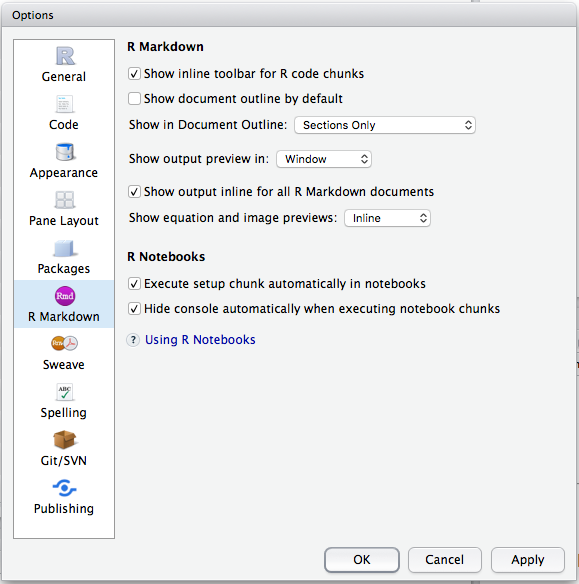
\includegraphics[width=0.9\linewidth]{images/rmd_window} 

}

\caption{To read RMarkdown output in a separate page (highly recommended for laptops) choose "RMarkdown" on the left and choose "Window" from the dropdown menu, and click OK.}\label{fig:rmd-window}
\end{figure}

\subsubsection{Opening RStudio Projects from the OS (by clicking in the
Finder)}\label{opening-rstudio-projects-from-the-os-by-clicking-in-the-finder}

\begin{itemize}
\tightlist
\item
  You can open an RStudio project by double clicking the RStudio Project
  icon from, for example, a Mac Finder window. It lives in a directory
  of the same name (but it has a \texttt{.Rproj} exension.)
\item
  Or if you are a command line type, use, for example
  \texttt{open\ my\_project.Rproj} from the Terminal.
\item
  You can open as many RStudio projects as you like at a time.
\item
  Each RStudio project launches its own, completely separate R session!
\item
  Interestingly, if you click on the \texttt{.Rproj} file of a project
  that is open, RStudio will open another instance of that project. So,
  don't click on the \texttt{.Rproj} file for a project that is already
  open!

  \begin{itemize}
  \tightlist
  \item
    (In other applications on the Mac that will typically just take you
    to the currently open docuemnt, but not so with RStudio.)
  \end{itemize}
\item
  Use cmd-TAB to switch between open RStudio projects.
\end{itemize}

\subsubsection{Opening RStudio Projects from
RStudio}\label{opening-rstudio-projects-from-rstudio}

\begin{itemize}
\tightlist
\item
  When you open existing projects using the ``File-\textgreater{}Open
  Project\ldots{}'' menu option or with the ``File -\textgreater{}
  Recent Projects'' menu option and you currently have RStudio open ``in
  another project,''" then the new project that you are opening jumps in
  ``on top of'' the previous one. It looks like your previous project
  has vanished into the ether. The OS thinks there is only one RStudio
  open, an it has the most recently opened project in it. WHERE'S MY
  OTHER ONE?!
\item
  You can get back to it by clicking the project dropdown in the upper
  right of the project.
\item
  However, if you switch between projects this way it restarts R each
  time you switch back to your project so it takes a lot of time and it
  is super-annoying.
\item
  If you are working concurrently in multiple projects, I recommend
  opening them from the Finder (or Terminal) and switching between them
  using \textbf{Cmd-TAB}.
\end{itemize}

\subsubsection{\texorpdfstring{What is the \texttt{.Rproj} file,
really}{What is the .Rproj file, really}}\label{what-is-the-.rproj-file-really}

It is just a text file that stores some information and any
project-specific preferences if there are any. Here is what
\texttt{rep-res-eeb-2017.Rproj} looks like if you open it with a text
editor:

\begin{Shaded}
\begin{Highlighting}[]
\FunctionTok{Version:} \NormalTok{1.0}

\FunctionTok{RestoreWorkspace:} \NormalTok{Default}
\FunctionTok{SaveWorkspace:} \NormalTok{Default}
\FunctionTok{AlwaysSaveHistory:} \NormalTok{Default}

\FunctionTok{EnableCodeIndexing:} \NormalTok{Yes}
\FunctionTok{UseSpacesForTab:} \NormalTok{Yes}
\FunctionTok{NumSpacesForTab:} \NormalTok{2}
\FunctionTok{Encoding:} \NormalTok{UTF-8}

\FunctionTok{RnwWeave:} \NormalTok{knitr}
\FunctionTok{LaTeX:} \NormalTok{pdfLaTeX}

\FunctionTok{AutoAppendNewline:} \NormalTok{Yes}
\FunctionTok{StripTrailingWhitespace:} \NormalTok{Yes}

\FunctionTok{BuildType:} \NormalTok{Website}
\end{Highlighting}
\end{Shaded}

\subsubsection{R in an RStudio project launches in the project
directory}\label{r-in-an-rstudio-project-launches-in-the-project-directory}

\begin{itemize}
\tightlist
\item
  This makes reproducibility much easier. You can find and load files
  using \emph{relative} paths.\\
\item
  Everything you might be accessing from R (data, scripts, etc.) or
  outputting from R will be easy to get to if they are ``in the
  project''
\item
  When we say that a file is ``in the project'' we mean that it is
  stored on disk somewhere within the project directory.
\item
  The project directory (sometimes called the \emph{root} of the project
  directory) is just the directory that contains the \texttt{.Rproj}
  file.
\item
  Expert user tip: \texttt{rprojroot::find\_rstudio\_root\_file()} (part
  of the \texttt{rprojroot} package) let's you find the root of an
  RStudio project directory. This can be helpful sometimes\ldots{}.
\end{itemize}

\subsection{Workflow: scripts}\label{workflow-scripts}

\begin{itemize}
\tightlist
\item
  Script editor window vs console window
\item
  Keyboard shortcuts for evaluating codes in your scripts:

  \begin{itemize}
  \tightlist
  \item
    \textbf{Cmd-Return} (sends current line to console and advances
    cursor to next line)
  \item
    \textbf{Highlight with Cmd-Return} (send highlighted code to
    console)

    \begin{itemize}
    \tightlist
    \item
      For this, \textbf{Shift-up-arrow} and \textbf{Shift-down-arrow}
      are good for highlighting.
    \item
      As is \textbf{Shift-Command-right-arrow} or
      \textbf{Shift-command-left-arrow}.
    \end{itemize}
  \end{itemize}
\end{itemize}

\section{\texorpdfstring{Let's talk about the pipe
\texttt{\%\textgreater{}\%}}{Let's talk about the pipe \%\textgreater{}\%}}\label{lets-talk-about-the-pipe}

For anyone who had ever worked comfortably in Unix for a long time, and
was used to chaining the output of one utility in as the input for
another utility using the pipe: \texttt{\textbar{}}, R's syntax for
composition of functions was always super cumbersome and required all
sorts of nasty, nested parentheses.

Consider this simple set of operations: imagine we want to

\begin{enumerate}
\def\labelenumi{\arabic{enumi}.}
\tightlist
\item
  simulate 1000 gamma random variables, \(G\), with parameters
  \(\alpha=5\) and \(\beta = 1\),
\item
  for each \(G\) simulate a Poisson random variable with mean
  (\texttt{lambda}) \(G\).
\item
  take the \texttt{sqrt} of each such variable
\item
  compute the variance of the result
\end{enumerate}

This can all be done in one line, but is ugly!

\begin{Shaded}
\begin{Highlighting}[]
\CommentTok{# set random seed for reproducibility}
\KeywordTok{set.seed}\NormalTok{(}\DecValTok{5}\NormalTok{)}

\KeywordTok{var}\NormalTok{(}\KeywordTok{sqrt}\NormalTok{(}\KeywordTok{rpois}\NormalTok{(}\DataTypeTok{n =} \DecValTok{1000}\NormalTok{, }\DataTypeTok{lambda =} \KeywordTok{rgamma}\NormalTok{(}\DataTypeTok{n =} \DecValTok{1000}\NormalTok{, }\DataTypeTok{shape =} \DecValTok{5}\NormalTok{, }\DataTypeTok{scale =} \DecValTok{1}\NormalTok{))))}
\end{Highlighting}
\end{Shaded}

\begin{verbatim}
## [1] 0.5828768
\end{verbatim}

It doesn't matter how stylishly you include spaces in your code, this is
just Fugly!

You can write it on multiple lines, but it is friggin' ghastly! Maybe
worse than before.

\begin{Shaded}
\begin{Highlighting}[]
\KeywordTok{set.seed}\NormalTok{(}\DecValTok{5}\NormalTok{)}

\KeywordTok{var}\NormalTok{(}
  \KeywordTok{sqrt}\NormalTok{(}
    \KeywordTok{rpois}\NormalTok{(}\DataTypeTok{n =} \DecValTok{1000}\NormalTok{, }\DataTypeTok{lambda =} \KeywordTok{rgamma}\NormalTok{(}
      \DataTypeTok{n =} \DecValTok{1000}\NormalTok{, }\DataTypeTok{shape =} \DecValTok{5}\NormalTok{, }\DataTypeTok{scale =} \DecValTok{1}
    \NormalTok{)}
    \NormalTok{)}
  \NormalTok{)}
\NormalTok{)}
\end{Highlighting}
\end{Shaded}

\begin{verbatim}
## [1] 0.5828768
\end{verbatim}

The problem is that the order in which the operations are done does not
match the way things are written: the first thing to get done is the
call to \texttt{rgamma}, which is nested deeply within the parentheses.

Enter the R ``pipe'' symbol. It is not as convenient to type as
\texttt{\textbar{}}, but you can make it quickly with the keyboard
shortcut \texttt{cmd-shift-M}: \texttt{\%\textgreater{}\%}. This was
introduced in the \texttt{magrittr} package, and the \texttt{tidyverse}
imports the \texttt{\%\textgreater{}\%} symbol from \texttt{magrittr}.

Behold!

\begin{Shaded}
\begin{Highlighting}[]
\KeywordTok{library}\NormalTok{(tidyverse)}
\KeywordTok{set.seed}\NormalTok{(}\DecValTok{5}\NormalTok{)}

\KeywordTok{rgamma}\NormalTok{(}\DataTypeTok{n =} \DecValTok{1000}\NormalTok{, }\DataTypeTok{shape =} \DecValTok{5}\NormalTok{, }\DataTypeTok{scale =} \DecValTok{1}\NormalTok{) %>%}
\StringTok{  }\KeywordTok{rpois}\NormalTok{(}\DataTypeTok{n =} \DecValTok{1000}\NormalTok{, }\DataTypeTok{lambda =} \NormalTok{.) %>%}\StringTok{          }\CommentTok{# pass G is as the lambda parameter using the dot: .}
\StringTok{  }\KeywordTok{sqrt}\NormalTok{() %>%}\StringTok{                               }\CommentTok{# no dot here, so the previous result is just the first argument to sqrt}
\StringTok{  }\KeywordTok{var}\NormalTok{()                                    }\CommentTok{# same here}
\end{Highlighting}
\end{Shaded}

\begin{verbatim}
## [1] 0.5828768
\end{verbatim}

That is a hell of a lot easier to read! It gives me goose bumps it is so
elegant.

The \texttt{\%\textgreater{}\%} symbol says, ``take the result that
occurred before the \texttt{\%\textgreater{}\%} and pass it in as the
\texttt{.} in whatever follows the \texttt{\%\textgreater{}\%}.''
Furthermore, if there is no \texttt{.} in the expression after the
\texttt{\%\textgreater{}\%}, simply pass the result that occurred before
the \texttt{\%\textgreater{}\%} in as the \emph{first argument} in the
function call that comes after the \texttt{\%\textgreater{}\%}.

This type of ``chaining'' of operations is particularly powerful when
operating on \texttt{tibbles} using \texttt{dplyr}

\section{\texorpdfstring{Tibbles and ``rectangular''
data}{Tibbles and rectangular data}}\label{tibbles-and-rectangular-data}

\begin{itemize}
\tightlist
\item
  gonna talk a little about data types too.
\item
  Chinook CWT data example.
\item
  Get comfy with the \texttt{View()} function!
\end{itemize}

\subsection{Tibble excercises}\label{tibble-excercises}

I'm gonna just blast through these here in case people are curious.
These are answers I would use.

\begin{enumerate}
\def\labelenumi{\arabic{enumi}.}
\item
  Use \texttt{class()}

\begin{Shaded}
\begin{Highlighting}[]
\KeywordTok{class}\NormalTok{(mtcars)}
\end{Highlighting}
\end{Shaded}

\begin{verbatim}
## [1] "data.frame"
\end{verbatim}

\begin{Shaded}
\begin{Highlighting}[]
\KeywordTok{class}\NormalTok{(tibble::}\KeywordTok{as_tibble}\NormalTok{(mtcars))}
\end{Highlighting}
\end{Shaded}

\begin{verbatim}
## [1] "tbl_df"     "tbl"        "data.frame"
\end{verbatim}

  Hey! does everyone see the \texttt{tibble::as\_tibble()} there? The
  \texttt{::} is the ``namespace addresser''. It lets you run a function
  from a library without loading the library. If you already have done
  \texttt{library(tidyverse)} you would have loaded the \texttt{tibble}
  library and could just write \texttt{as\_tibble(mtcars)} but I wanted
  to be explicit about where the \texttt{as\_tibble()} function comes
  from. (As an aside, it turns out that this is how you would write it
  if you were writing code for a package.)
\item
  Let's do it first as a \texttt{data.frame}:

\begin{Shaded}
\begin{Highlighting}[]
\KeywordTok{library}\NormalTok{(tidyverse)}
\NormalTok{df <-}\StringTok{ }\KeywordTok{data.frame}\NormalTok{(}\DataTypeTok{abc =} \DecValTok{1}\NormalTok{, }\DataTypeTok{xyz =} \StringTok{"a"}\NormalTok{)}
\NormalTok{df$x}
\end{Highlighting}
\end{Shaded}

\begin{verbatim}
## [1] a
## Levels: a
\end{verbatim}

\begin{Shaded}
\begin{Highlighting}[]
\NormalTok{df[, }\StringTok{"xyz"}\NormalTok{]}
\end{Highlighting}
\end{Shaded}

\begin{verbatim}
## [1] a
## Levels: a
\end{verbatim}

\begin{Shaded}
\begin{Highlighting}[]
\NormalTok{df[, }\KeywordTok{c}\NormalTok{(}\StringTok{"abc"}\NormalTok{, }\StringTok{"xyz"}\NormalTok{)]}
\end{Highlighting}
\end{Shaded}

\begin{verbatim}
##   abc xyz
## 1   1   a
\end{verbatim}

  And then we can do it again as a \texttt{tibble}

\begin{Shaded}
\begin{Highlighting}[]
\NormalTok{df <-}\StringTok{ }\KeywordTok{tibble}\NormalTok{(}\DataTypeTok{abc =} \DecValTok{1}\NormalTok{, }\DataTypeTok{xyz =} \StringTok{"a"}\NormalTok{) %>%}
\StringTok{  }\KeywordTok{as_tibble}\NormalTok{()}
\NormalTok{df$x}
\end{Highlighting}
\end{Shaded}

\begin{verbatim}
## Warning: Unknown column 'x'
\end{verbatim}

\begin{verbatim}
## NULL
\end{verbatim}

\begin{Shaded}
\begin{Highlighting}[]
\NormalTok{df$xyz}
\end{Highlighting}
\end{Shaded}

\begin{verbatim}
## [1] "a"
\end{verbatim}

\begin{Shaded}
\begin{Highlighting}[]
\NormalTok{df[, }\StringTok{"xyz"}\NormalTok{]}
\end{Highlighting}
\end{Shaded}

\begin{verbatim}
## # A tibble: 1 × 1
##     xyz
##   <chr>
## 1     a
\end{verbatim}

\begin{Shaded}
\begin{Highlighting}[]
\NormalTok{df[, }\KeywordTok{c}\NormalTok{(}\StringTok{"abc"}\NormalTok{, }\StringTok{"xyz"}\NormalTok{)]}
\end{Highlighting}
\end{Shaded}

\begin{verbatim}
## # A tibble: 1 × 2
##     abc   xyz
##   <dbl> <chr>
## 1     1     a
\end{verbatim}

  Aha! Things to notice are:

  \begin{enumerate}
  \def\labelenumii{\alph{enumii}.}
  \tightlist
  \item
    \texttt{data.frame()} coerces to factors.
  \item
    tibble doesn't do partial name matching
    \texttt{\$x}\(\neq\)\texttt{\$xyz}
  \item
    Square bracket extraction of a single column of a tibble retains its
    tibbleness. Not so with \texttt{data.frame}. With
    \texttt{data.frame} it gets turned into a vector.
  \item
    \texttt{\$} extraction with \texttt{tibble} returns a vector.
  \end{enumerate}
\item
  Let's make \texttt{mtcars} a \texttt{tibble}

\begin{Shaded}
\begin{Highlighting}[]
\NormalTok{mtcars_t <-}\StringTok{ }\KeywordTok{as_tibble}\NormalTok{(mtcars)}
\NormalTok{var <-}\StringTok{ "mpg"}

\CommentTok{# this will get the "mpg" column out but retain it as a tibble}
\NormalTok{mtcars_t[, var]}
\end{Highlighting}
\end{Shaded}

\begin{verbatim}
## # A tibble: 32 × 1
##      mpg
##    <dbl>
## 1   21.0
## 2   21.0
## 3   22.8
## 4   21.4
## 5   18.7
## 6   18.1
## 7   14.3
## 8   24.4
## 9   22.8
## 10  19.2
## # ... with 22 more rows
\end{verbatim}

\begin{Shaded}
\begin{Highlighting}[]
\CommentTok{# and this will just grab the column as a vector}
\NormalTok{mtcars_t[[var]]}
\end{Highlighting}
\end{Shaded}

\begin{verbatim}
##  [1] 21.0 21.0 22.8 21.4 18.7 18.1 14.3 24.4 22.8 19.2 17.8 16.4 17.3 15.2
## [15] 10.4 10.4 14.7 32.4 30.4 33.9 21.5 15.5 15.2 13.3 19.2 27.3 26.0 30.4
## [29] 15.8 19.7 15.0 21.4
\end{verbatim}
\item
  Remember that non-syntactic names (those that do not start with a
  letter or underscore and which include characters other than
  \texttt{-} and ``\_" and ``.'') must be enclosed in backticks. Let's
  get our data:

\begin{Shaded}
\begin{Highlighting}[]
\NormalTok{annoying <-}\StringTok{ }\KeywordTok{tibble}\NormalTok{(}
\StringTok{`}\DataTypeTok{1}\StringTok{`} \NormalTok{=}\StringTok{ }\DecValTok{1}\NormalTok{:}\DecValTok{10}\NormalTok{,}
\StringTok{`}\DataTypeTok{2}\StringTok{`} \NormalTok{=}\StringTok{ `}\DataTypeTok{1}\StringTok{`} \NormalTok{*}\StringTok{ }\DecValTok{2} \NormalTok{+}\StringTok{ }\KeywordTok{rnorm}\NormalTok{(}\KeywordTok{length}\NormalTok{(}\StringTok{`}\DataTypeTok{1}\StringTok{`}\NormalTok{))}
\NormalTok{)}
\end{Highlighting}
\end{Shaded}

  OK, now let's do the questions:

  \begin{enumerate}
  \def\labelenumii{\arabic{enumii}.}
  \item
    Use dollar sign with backticks:

\begin{Shaded}
\begin{Highlighting}[]
\NormalTok{annoying$}\StringTok{`}\DataTypeTok{1}\StringTok{`}
\end{Highlighting}
\end{Shaded}

\begin{verbatim}
##  [1]  1  2  3  4  5  6  7  8  9 10
\end{verbatim}
  \item
    Use dollar sign with backticks

\begin{Shaded}
\begin{Highlighting}[]
\KeywordTok{plot}\NormalTok{(annoying$}\StringTok{`}\DataTypeTok{1}\StringTok{`}\NormalTok{, annoying$}\StringTok{`}\DataTypeTok{2}\StringTok{`}\NormalTok{)}
\end{Highlighting}
\end{Shaded}

    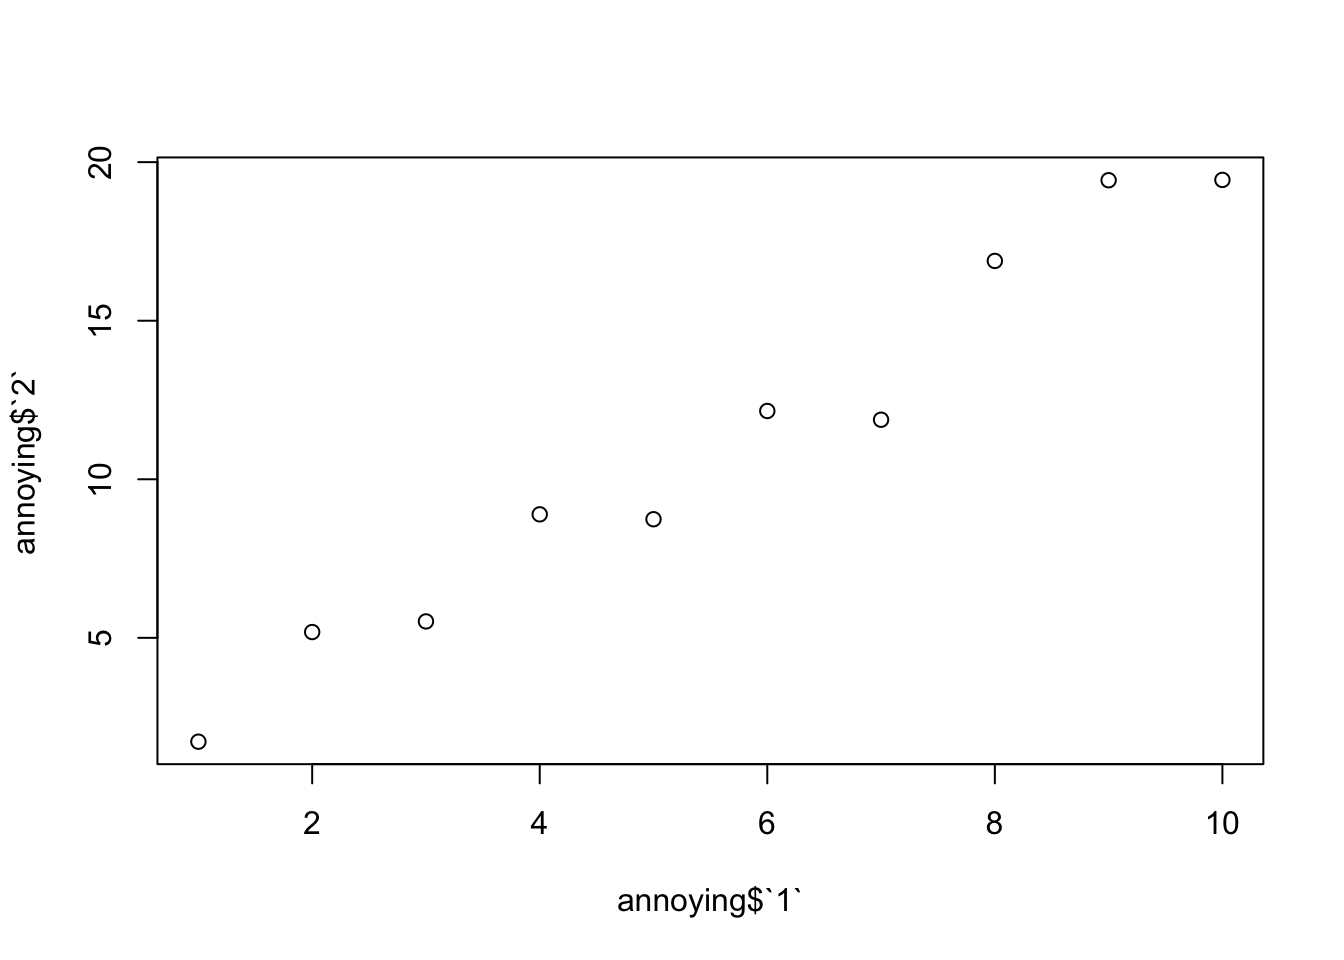
\includegraphics{bookdown-demo_files/figure-latex/unnamed-chunk-10-1.pdf}
  \item
    Use \texttt{mutate} (we haven't talked about this yet) with
    backticks

\begin{Shaded}
\begin{Highlighting}[]
\NormalTok{annoying %>%}
\StringTok{  }\KeywordTok{mutate}\NormalTok{(}\StringTok{`}\DataTypeTok{3}\StringTok{`} \NormalTok{=}\StringTok{ `}\DataTypeTok{2}\StringTok{`} \NormalTok{/}\StringTok{ `}\DataTypeTok{1}\StringTok{`}\NormalTok{)}
\end{Highlighting}
\end{Shaded}

\begin{verbatim}
## # A tibble: 10 × 3
##      `1`       `2`      `3`
##    <int>     <dbl>    <dbl>
## 1      1  1.725450 1.725450
## 2      2  5.182598 2.591299
## 3      3  5.517888 1.839296
## 4      4  8.894382 2.223596
## 5      5  8.740021 1.748004
## 6      6 12.153600 2.025600
## 7      7 11.878134 1.696876
## 8      8 16.885478 2.110685
## 9      9 19.429848 2.158872
## 10    10 19.439987 1.943999
\end{verbatim}
  \item
    Use \texttt{rename} (we haven't talked about this yet) with
    backticks

\begin{Shaded}
\begin{Highlighting}[]
\NormalTok{annoying %>%}
\StringTok{  }\KeywordTok{mutate}\NormalTok{(}\StringTok{`}\DataTypeTok{3}\StringTok{`} \NormalTok{=}\StringTok{ `}\DataTypeTok{2}\StringTok{`} \NormalTok{/}\StringTok{ `}\DataTypeTok{1}\StringTok{`}\NormalTok{) %>%}
\StringTok{  }\KeywordTok{rename}\NormalTok{(}\DataTypeTok{one =} \StringTok{`}\DataTypeTok{1}\StringTok{`}\NormalTok{, }
         \DataTypeTok{two =} \StringTok{`}\DataTypeTok{2}\StringTok{`}\NormalTok{,}
         \DataTypeTok{three =} \StringTok{`}\DataTypeTok{3}\StringTok{`}\NormalTok{)}
\end{Highlighting}
\end{Shaded}

\begin{verbatim}
## # A tibble: 10 × 3
##      one       two    three
##    <int>     <dbl>    <dbl>
## 1      1  1.725450 1.725450
## 2      2  5.182598 2.591299
## 3      3  5.517888 1.839296
## 4      4  8.894382 2.223596
## 5      5  8.740021 1.748004
## 6      6 12.153600 2.025600
## 7      7 11.878134 1.696876
## 8      8 16.885478 2.110685
## 9      9 19.429848 2.158872
## 10    10 19.439987 1.943999
\end{verbatim}
  \end{enumerate}
\item
  Look it up with \texttt{?enframe}. It turns out that
  \texttt{enframe()} is super useful.\\
  Often you will have a vector of values with names associated with it.
  For example:

\begin{Shaded}
\begin{Highlighting}[]
\NormalTok{v <-}\StringTok{ }\KeywordTok{c}\NormalTok{(}\DecValTok{1}\NormalTok{, }\DecValTok{3}\NormalTok{, }\DecValTok{4}\NormalTok{, }\DecValTok{10}\NormalTok{)}
\KeywordTok{names}\NormalTok{(v) <-}\StringTok{ }\KeywordTok{c}\NormalTok{(}\StringTok{"a"}\NormalTok{, }\StringTok{"b"}\NormalTok{, }\StringTok{"b"}\NormalTok{, }\StringTok{"c"}\NormalTok{)}
\NormalTok{v}
\end{Highlighting}
\end{Shaded}

\begin{verbatim}
##  a  b  b  c 
##  1  3  4 10
\end{verbatim}

  If you want to deal with this type of vector in the tidyverse, you can
  enframe it into a tibble:

\begin{Shaded}
\begin{Highlighting}[]
\KeywordTok{enframe}\NormalTok{(v)}
\end{Highlighting}
\end{Shaded}

\begin{verbatim}
## # A tibble: 4 × 2
##    name value
##   <chr> <dbl>
## 1     a     1
## 2     b     3
## 3     b     4
## 4     c    10
\end{verbatim}

  By default it makes columns of ``name'' and ``value''. That is
  awesome!
\item
  Do \texttt{package?tibble} and read through it to find that the answer
  we want is \texttt{tibble.max\_extra\_cols}.
\end{enumerate}

\section{Data import}\label{data-import}

\begin{itemize}
\tightlist
\item
  Why use \texttt{readr} instead of the base-R reading functions? Plenty
  of reasons.
\item
  Explicit column specifications if you want to do that.
\end{itemize}

\subsection{RStudio's GUI importer}\label{rstudios-gui-importer}

\begin{itemize}
\tightlist
\item
  This is a great way to start importing CSV files.
\item
  Don't do it every time! use the code that it creates to make reading
  your data in reproducible.
\end{itemize}

\chapter{Week Three Meeting}\label{week3}

\section{Git Basics}\label{git-basics}

Goals for Today:

\begin{itemize}
\tightlist
\item
  Explain what git is (and how it is different than GitHub)
\item
  Introduce the sha-1 hash (for fun!)
\item
  Get familiar with RStudio's very convenient interface to git

  \begin{itemize}
  \tightlist
  \item
    staging files
  \item
    unstaging file
  \item
    viewing differences between staged and unstaged files
  \item
    committing files
  \item
    viewing the commit history
  \end{itemize}
\end{itemize}

\subsection{An overview of Version Control Systems (VCS)}\label{vcs}

\begin{itemize}
\tightlist
\item
  Git is a type of VCS
\item
  At its crudest, a VCS is a system that provides a way of saving and
  restoring earlier versions of a file.
\end{itemize}

\subsubsection{A typical VCS for a non-computer
programmer}\label{a-typical-vcs-for-a-non-computer-programmer}

\begin{itemize}
\tightlist
\item
  Start writing \texttt{my\_manuscript.doc}.
\item
  At some point worry that MS Word is going to eat your file, so,

  \begin{itemize}
  \tightlist
  \item
    Make a ``backup'' called \texttt{my\_manuscript\_A.doc}
  \end{itemize}
\item
  Then, before overhauling the discussion, save the current file as
  \texttt{my\_manuscript\_B.doc}.
\item
  Email it to your coauthors and then have a series of files with other
  extensions such as the initials of their names when they edit them and
  send them back.
\item
  Etc.
\item
  Disadvantages:

  \begin{itemize}
  \tightlist
  \item
    Hard to find a good record of what is in each version. (Wait! I
    liked the introduction I wrote three weeks ago\ldots{}where is that
    now?)
  \item
    A terrible system if you have multiple files that are dependent on
    one another (for example, figures in your document, or scripts and
    data sets if you have a programming project.)
  \item
    If you decide that you want to merge the changes you made to the
    discussion in version \texttt{\_C} with the edits on the
    introduction in version \texttt{\_K}, it is hard.
  \end{itemize}
\end{itemize}

\subsubsection{Other popular VCS
systems}\label{other-popular-vcs-systems}

\begin{itemize}
\tightlist
\item
  rcs, cvs, subversion, etc.
\item
  These all had a ``Centralized'' model:

  \begin{itemize}
  \tightlist
  \item
    You set up a repository on a server that has the full version
    history,
  \item
    then each person working on it gets a copy of the current version,
    and nothing more.
  \item
    They can submit changes back to the central repository which tries
    to deal with conflicting submissions.
  \item
    You need to be online to do most operations.
  \end{itemize}
\item
  I used a few of these, and missed them for a few weeks when I switched
  to Git, but then never looked back and couldn't imagine using them
  again.
\end{itemize}

\subsubsection{The Git model --- Distributed Version
Control}\label{the-git-model-distributed-version-control}

\begin{itemize}
\tightlist
\item
  Git stores ``snapshots'' of your collection of files in a repository
\item
  For our work, the ``collection of files'' will be ``the stuff in your
  RStudio project''

  \begin{itemize}
  \tightlist
  \item
    Another reason it is nice to keep everything you need for a project
    together in a ``project directory''
  \item
    Though git scans your project directory for new additions and
    changes, it will not add a new file, or add new changes, to the
    repository until you \emph{stage} and subsequently \emph{commit} the
    file.
  \end{itemize}
\item
  When you clone a repository, \textbf{you} get the whole version
  history
\item
  When someone else clones that repository, \textbf{they also} get the
  whole version history.
\item
  Git has well-developed features for merging changes made in different
  repositories

  \begin{itemize}
  \tightlist
  \item
    But, for today, we will talk mostly of a single user interacting
    with git.
  \end{itemize}
\end{itemize}

\subsection{Git versus GitHub}\label{git-versus-github}

\begin{itemize}
\tightlist
\item
  They are not the same thing!
\item
  Git is software that you can run on your own machine for doing version
  control on a repository.

  \begin{itemize}
  \tightlist
  \item
    It can be \emph{entirely} local. i.e.~only on your hard drive and
    nowhere else.
  \item
    This is super-useful for any project, because solid version control
    is great to have.
  \end{itemize}
\item
  GitHub is a website, with tools powered by Git (and many that they
  brewed up themselves) that makes it very, very easy to share git
  repositories with people all over the place.
\end{itemize}

\subsubsection{Is everything on GitHub
public?}\label{is-everything-on-github-public}

\begin{itemize}
\tightlist
\item
  No! Many companies use GitHub to host their proprietary code

  \begin{itemize}
  \tightlist
  \item
    They just have to pay for that\ldots{}
  \end{itemize}
\item
  By default, you can put anything on GitHub for free as long as it is
  under a fairly free-use (open source type) license and it is available
  to anyone
\item
  If you want a private repository, as an academic affiliate you just
  have to ask and GitHub will give you unlimited private repos for free.
\item
  And if you are a student and you have not yet done so, go to
  \url{https://education.github.com/pack} to sign up for your free
  student pack.
\end{itemize}

\subsection{Using git through RStudio}\label{git-thru-rstudio}

\begin{itemize}
\tightlist
\item
  Now we can do a few things together to see how this works.
\item
  Most of the action is in the Git Pane\ldots{}
\item
  Today we will talk about:

  \begin{itemize}
  \tightlist
  \item
    Staging files (preparing them to be \textbf{committed})
  \item
    Committing files (putting them into the repository)
  \item
    viewing differences between staged and unstaged files
  \item
    committing files
  \item
    viewing the commit history
  \end{itemize}
\end{itemize}

\subsubsection{Two final configurations before
starting:}\label{two-final-configurations-before-starting}

\begin{itemize}
\item
  Open the shell (Tools-\textgreater{}Shell\ldots{}) and issue these two
  commands, replacing the name ``John Doe'' with yours, and his email
  with yours.

  \begin{itemize}
  \item
    You may as well use the email address that you gave to GitHub,
    though it doesn't necessarily have to be

\begin{verbatim}
git config --global user.name "John Doe"
git config --global user.email johndoe@example.com
\end{verbatim}

    You only need to do this once.
  \end{itemize}
\item
  Finally, if you are using a Mac, configure it to cache your GitHub
  credentials so you needn't give your password every time you push to
  it:

\begin{verbatim}
git config --global credential.helper osxkeychain
\end{verbatim}
\end{itemize}

\subsubsection{The status/staging panel}\label{the-statusstaging-panel}

\begin{itemize}
\tightlist
\item
  RStudio keeps git constantly scanning the project directory to find
  any files that have changed or which are new.
\item
  By clicking a file's little ``check-box'' you can stage it.\\
\item
  Some symbols:

  \begin{itemize}
  \tightlist
  \item
    \textbf{Blue-M}: a file that is already under version control that
    has been modified.
  \item
    \textbf{Yellow-?}: a file that is not under version control
    (yet\ldots{})
  \item
    \textbf{Green-A}: a file that was not under version control, but
    which has been staged to be committed.
  \item
    \textbf{Red-D}: a file under version control has been deleted. To
    make it really disappear, you have to stage its disappearance and
    commit. Note that it still lives on, but you have to dig back into
    your history to find it.
  \item
    \textbf{Purple-R} a file that was renamed. (Note that git in Rstudio
    seems to be figuring this out on its own.)
  \end{itemize}
\end{itemize}

\subsubsection{The Diff window}\label{the-diff-window}

\begin{itemize}
\tightlist
\item
  Shows what has changed between the last committed version of a file
  and its current state.
\item
  Holy smokes this is convenient
\item
  (Note: all this output is available from the command line, but the
  Rstudio interface is very nice, IMHO)
\end{itemize}

\subsubsection{Making a Commit}\label{making-a-commit}

\begin{itemize}
\tightlist
\item
  Super easy:

  \begin{itemize}
  \tightlist
  \item
    After staging the files you want to commit\ldots{}
  \item
    Write a brief message (first line short, then as much after that as
    you want) and hit the commit button.
  \end{itemize}
\end{itemize}

\subsubsection{The History window}\label{the-history-window}

\begin{itemize}
\tightlist
\item
  Easy inspection of past commits.
\item
  See what changes were made at each commit.
\end{itemize}

\subsection{Go for it everyone!}\label{git-play}

\begin{itemize}
\tightlist
\item
  Make some changes and commit them yourselves.\\
\item
  Add some new files to the project, and commit those.
\item
  Get familiar with the diff window.
\item
  Check the history after a few commits.
\end{itemize}

\subsection{How does git store and keep track of things}\label{git-how}

\begin{itemize}
\tightlist
\item
  Everything is stored in the .git folder inside the RStudio project.
\item
  The ``working copy'' gets checkout out of there
\item
  Committed changes are recorded to the directory
\end{itemize}

\subsubsection{What is inside of the .git
directory?}\label{what-is-inside-of-the-.git-directory}

We can use R to list the files. My \texttt{rep-res-course} repository
that hold all the materials for a course like this one looks like:

\begin{Shaded}
\begin{Highlighting}[]
\NormalTok{## check out this file-system command in R}
\KeywordTok{dir}\NormalTok{(}\DataTypeTok{path =} \StringTok{".git"}\NormalTok{, }\DataTypeTok{all.files =} \OtherTok{TRUE}\NormalTok{, }\DataTypeTok{recursive =} \OtherTok{TRUE}\NormalTok{)}
\end{Highlighting}
\end{Shaded}

The output from that command looks something like this:

\begin{verbatim}
  [1] "#MERGE_MSG#"                                       "COMMIT_EDITMSG"                                   
  [3] "COMMIT_EDITMSG~"                                   "config"                                           
  [5] "description"                                       "FETCH_HEAD"                                       
  [7] "HEAD"                                              "hooks/applypatch-msg.sample"                      
  [9] "hooks/commit-msg.sample"                           "hooks/post-update.sample"                         
 [11] "hooks/pre-applypatch.sample"                       "hooks/pre-commit.sample"                          
 [13] "hooks/pre-push.sample"                             "hooks/pre-rebase.sample"                          
 [15] "hooks/prepare-commit-msg.sample"                   "hooks/update.sample"                              
 [17] "index"                                             "info/exclude"                                     
 [19] "logs/HEAD"                                         "logs/refs/heads/gh-pages"                         
 [21] "logs/refs/heads/master"                            "logs/refs/remotes/origin/gh-pages"                
 [23] "logs/refs/remotes/origin/master"                   "objects/00/906f99e192ff64b4e9e9a0e5745b0a4f841cbd"
 [25] "objects/01/ab18d4ce04fb06532bb06ed579218fef89d478" "objects/02/74554e0b574b9beb2144f26ad3925830056870"
 [27] "objects/03/2d224bf78798e8b9765af6d8768ade14694a9d" "objects/04/03d552ab37b0bcaeebed0ac3068d669261c456"
 [29] "objects/04/4a12f8ccc12a4a5ba84ab2bf5a1ae751feea6f" "objects/04/9ec3065bb0434ded671fa83af5ade803bc11a1"
 [31] "objects/04/ea8efb1367727b081dea87e63818be0a4d02f0" "objects/05/b22ecc373d5058e36d7ca773a4475c46daef77"
 [33] "objects/07/8831b46c9b63e8c2d50b79304ed05de9274c28" "objects/07/b57af2a0cbd0545a6cd3e93f10cc5d768e42ba"
 [35] "objects/08/674e6e4d534b3424e2629510d20bb6d1b0be94" "objects/08/8b282d5b978dc1ff6eef3871d3fb3a9256246a"
 [37] "objects/09/565dcd10d7adc0551783b443e8fd71486b3997" "objects/09/6828a0cfb96f30d6e99cfc04a5c1686b9e318c"
 [39] "objects/0a/30fe678abc342c58daab0ad42163b371babda0" "objects/0a/b71109dae6e5711755feddfb06b81b13766496"
 [41] "objects/0b/442fdfc183783537985c17151ae3483fa00cf6" "objects/0b/c0451fd0e7081a7db05fdd38b12870bdcabd13"
 [43] "objects/0c/0f7cf8c73d901795dad4bd5f504c53c3bf2093" "objects/0d/14a7a2a19ffc3b9820f011e3270c965a5fefce"
 [45] "objects/0e/35cfb4d55e52d27083b8d2eccab9296b920d76" "objects/0e/7bba5882077a8b00a76d3eabe6b23cadc658e6"
 [47] "objects/0e/8abf4cc0885a727ee2459fdbb272828e267cc4" "objects/0f/1f3f7be7787d5d44dc1155f3b7a44eddc9f0be"
 [49] "objects/10/54d2e7a9baf61618521c522b15db40855b3431" "objects/11/7d874e1616500b5fba51b9f0ee1e8d0fbe1dc2"
 [51] "objects/11/c33cc1d5c8de7c7cbf7257b7d32f7ca3d458ef" "objects/14/1ccea514e106e20eef47b791a23e036d1fa1d2"
 [53] "objects/15/cc3a6f15dadb3446ad0af34a3ecde8d81d65f9" "objects/15/ddaf45bf00c3ef2d8f499ebd6dc3a86bf9c3ab"
 [55] "objects/16/0c9386dfa9707d81fbbbcc52f0c7638703f9a9" "objects/16/8ee93b6a4612dbd76bc06a49460df9f9f6c41b"
\end{verbatim}

\textbf{Yikes!}

\subsubsection{How does git know a file has
changed?}\label{how-does-git-know-a-file-has-changed}

\begin{itemize}
\tightlist
\item
  Does it just look at the modification date?
\item
  NO! It ``fingerprints'' every file, so it knows when it has changed
  from the most recent committed version.

  \begin{itemize}
  \tightlist
  \item
    Demonstration. Change a file. Save, then undo the change and save
    again\ldots{}Git knows the file has been changed back to its
    ``former self''
  \end{itemize}
\item
  SHA-1 hashes. We will learn more about those later.\\
\item
  You will see things like
  \texttt{ed00c10ae6cf7bcc35d335d2edad7e71bc0f6770} all over in
  Git-land.
\item
  You can treat them as very specific names for different commits.
\end{itemize}

\subsubsection{What should I keep under version
control?}\label{what-should-i-keep-under-version-control}

\begin{itemize}
\tightlist
\item
  General rule: don't keep derived products.

  \begin{itemize}
  \tightlist
  \item
    i.e.~If you have an Rmd file that creates an html file, there isn't
    much need to put the html file under version control with git,
    because you can just regenerate it by Knitting the Rmd file.
  \end{itemize}
\item
  Do keep data, source code, etc.
\item
  Sometimes certain outputs and intermediate results from long
  calculations can be committed so that you don't have to run a 4 hour
  analysis to start where you were before.
\item
  For such results, consider \texttt{saveRDS()} with the
  \texttt{compress\ =\ "xz"} option (and its companion
  \texttt{readRDS()}.
\end{itemize}

\subsubsection{How can I make git ignore certain
files?}\label{how-can-i-make-git-ignore-certain-files}

\begin{itemize}
\tightlist
\item
  The \texttt{.gitignore} file!
\item
  File names (and patterns) in the \texttt{.gitignore} file are ignored
  \emph{recursively} (down into subdirectories), by default.
\item
  Files won't be ignored if they are already in the repository.
\item
  Example: \texttt{*.html}
\end{itemize}

\section{Pushing and Pulling With
GitHub}\label{pushing-and-pulling-with-github}

\subsection{Creating a Repository on GitHub and the initial
push}\label{creating-a-repository-on-github-and-the-initial-push}

When you have an RStudio project under git version control on your
laptop or desktop computer, creating a remote repository on GitHub is
quite easy. A few steps:

\begin{enumerate}
\def\labelenumi{\arabic{enumi}.}
\tightlist
\item
  Upper right corner: ``create new'' button (a ``+'' with a little
  triangle.) Choose ``New Repository''
\item
  Give it a name. It makes most sense to name it the same as the RStudio
  project you want to push up there. So, for example, if my project file
  was \texttt{boing.Rproj}, I would name the repository \texttt{boing}.
\item
  Add a 5 or 6 word description if you want.
\item
  Choose \textbf{public} or \textbf{private}
\item
  DO \textbf{NOT} choose to ``Initialize this repository with a
  README''. You likely already have a README. Initializing the
  repository with one will create headaches.
\item
  Also, don't add a \texttt{.gitignore} or a license (select ``none'',
  which should be the default, for both of those)
\item
  Click the green ``Create Repository'' button
\end{enumerate}

That will take you to another screen. In the middle find the code box
below the heading, \textbf{\ldots{}or push an existing repository from
the command line}.

\begin{enumerate}
\def\labelenumi{\arabic{enumi}.}
\item
  Copy that two lines of code from you web browser. It will look
  something like this:

\begin{verbatim}
git remote add origin https://github.com/eriqande/boing.git
git push -u origin master
\end{verbatim}

  but it will be specific to the repository you just made, so the URL
  and name of the repo will be different than what you see above. Note,
  you can copy the lines by clicking the ``copy this text'' icon on the
  right side of the page.
\item
  Go to RStudio, in the project that you want to push to GitHub, and
  choose ``Tools-Shell''. That will give you a terminal window. Paste
  the commands you copied into that terminal window and hit return.
\item
  It might ask you for your GitHub username and password.
\end{enumerate}

Voila!

\subsection{Subsequent pushes}\label{subsequent-pushes}

Once you have pushed the repo up there. Try making some changes on your
laptop, committing them, and then hitting the ``Push'' button on the git
panel\ldots{}

\subsection{Assign collaborators}\label{assign-collaborators}

From the repository page on GitHub, choose ``Settings'' (on the upper
right) and find the ``collaborators'' link (on the left).

If you have a private repository, you can add GitHub user
\texttt{eriqande} (that's me\ldots{}) to it and I will be able to view
it and give comments and suggestions.

\section{Next Week's Assignment}\label{next-weeks-assignment}

\begin{itemize}
\tightlist
\item
  With luck, we will get everyone's projects up to GitHub before the end
  of our session today. However, if we don't, please get that done ASAP.
\item
  The big assignment is to read the
  \href{http://r4ds.had.co.nz/transform.html}{Data Transformation}
  chapter in ``R for Data Science.'' \emph{Warning}: This is a long and
  meaty chapter, so get an early start! The chapter goes through what
  you need to know to leverage all the \texttt{dplyr} goodness. Please
  work all the examples, and do the exercises. In fact, when you are
  working through the examples with the \texttt{nycflights} data set,
  you should, after each example, try to do the same type of operation
  on your own data set.
\end{itemize}

\bibliography{packages.bib,book.bib}


\end{document}
